\documentclass[titlepage, 12pt, a4paper]{article}
\usepackage[utf8]{inputenc}
\usepackage{hyperref}
\usepackage{csquotes}
\usepackage{listings}
\usepackage{float}
\usepackage{graphicx}
\usepackage{mathptmx}
\usepackage{comment}
\usepackage[
backend=biber,
style=alphabetic,
sorting=ynt]{biblatex}
\usepackage{anysize}

% color in page
\usepackage{afterpage}
\usepackage{xcolor}
\usepackage{pagecolor}

% Margin sizes for page
\marginsize{3cm}{3cm}{2.5cm}{2.5cm}
 
\usepackage[nonumberlist,acronymlists={gloss}]{glossaries}
\makeglossaries

\newglossaryentry{latex}
{
	name=latex,
	description={A markup language}
}


\addbibresource{bibliography.bib}
\title{Doble factor de autenticación independiente de SO}
\author{Roselló Morell, Sergio\\
\texttt{sergio.rosello@live.u-tad.com}}

\begin{document}

\newpagecolor{blue}
\afterpage{\restorepagecolor}
\maketitle
\tableofcontents
\clearpage
\section{Agradecimientos}
Debo agradecer a Eduardo Ariols, mi tutor del trabajo todo el apoyo y consejos dados. Estoy seguro de que sin su ayuda, este trabajo no hubiese llegado a su nivel actual. Durante el proceso de elección del trabajo, me ayudó a darme cuenta de lo que quería hacer exactamente y desde ese momento, no ha parado de inspirarme con distintas formas de ver las cosas. De eso, le estoy muy agradecido.\\También quiero agradecer a la universidad el buen trabajo a la hora de escoger al personal docente de mi grado, puesto que en todo momento han demostrado más que profesionalidad y compañerismo hacia mi y mis compañeros de carrera.
\clearpage
\section{Resumen}
Este documento explica al lector la experiencia que he tenido durante el periodo de realización del trabajo de final de grado. Este trabajo trata sobre la autenticación de un usuario a un sistema \Gls{GNU/Linux}, en concreto, mediante una llave \Gls{USB}.\\Durante la fase de investigación de las tecnologías existentes, encontré algunas que ofrecían usa solución elegante, mediante \Gls{dbus} pero acabando la fase de investigación encontré un proyecto llamado \Gls{PAM} que redefinió la forma en la que planteaba el trabajo. Ésta es la forma por defecto de autenticar a los usuarios que tienen la mayoría de sistemas \Gls{GNU/Linux}.\\Este trabajo, al principio con enfoque mucho más práctico ha acabado teniendo un enfoque investigativo puesto que para implementar el módulo de autenticación, he tenido que construir una base fuerte sobre la que sentirme cómodo. Esta base es la que he tenido que esforzarme a entender puesto a que sin ella, el trabajo realizado, aunque funcionalmente completo, no me hubiese sido ni la mitad de estimulante e interesante.
\begin{abstract}
	This document reports my experience as I work on creating a USB-centric authentication method for \Gls{GNU/Linux}. During the research phase, I came across several elegant implementations, all of them worked with \Gls{dbus}. During the final stages of this period, I discovered \Gls{PAM} which changed my whole perspective on this project. Most of \Gls{GNU/Linux} systems use this module to enable authentication for their users.\\At the start of this project I would've expected to code a lot more, but now I realise that without a solid foundation, I may have been able to do what I had proposed, but I would not have the understanding on how the \Gls{PAM} fits into the whole equation and the many benefits it provides. This, I think is the point of this work.
\end{abstract}
\clearpage
\listoffigures
\clearpage
\printglossary[title={Abreviaciones y tecnicismos}]
\clearpage
\section{Estado del arte}
\subsection{Evolución de las tecnologías}
Los ordenadores forman una gran parte de nuestra sociedad desde que fueron inventados. El primer ordenador que se creó fue el Mark I, en 1944. Este ordenador estaba hecho mayoritariamente para realizar cálculos, pesaba cinco toneladas y se sobrecalentaba.
Desde Mark I, como podemos observar en la imagen \ref{fig:moore}, los ordenadores han ido duplicando el número de transistores en circuitos integrados cada dos años \cite{moore}. Hasta ahora, y seguramente unos años más en adelante, podamos ver que se sigue cumpliendo la ley de Moore.
\begin{figure}[H]
    \centering
    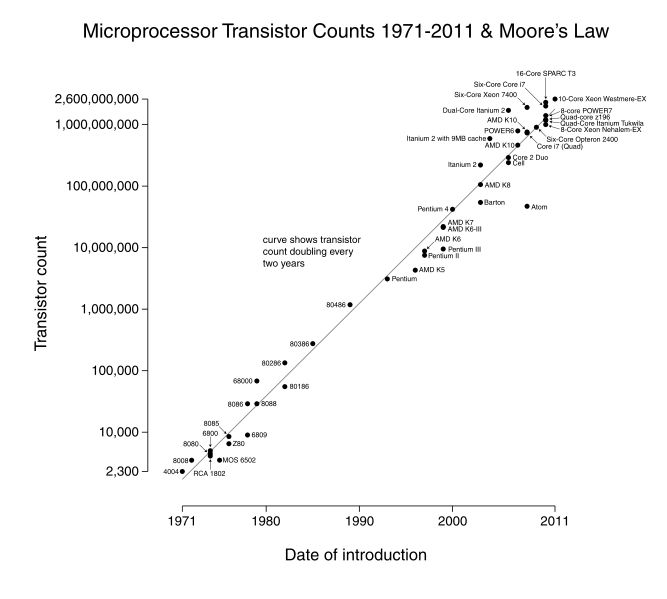
\includegraphics[width=0.5\textwidth]{Media/moore.jpg}
    \caption{Ley de Moore}
    \label{fig:moore}
\end{figure}
Durante el periodo de evolución de la informática, se pueden diferenciar cinco generaciones:
\begin{itemize}
	\item{\textbf{Primera generación: }}Estos ordenadores no se parecían en nada a los ordenadores modernos, eran extremadamente grandes y poco sofisticados. Eran estructuras tan grandes como una habitación entera y usaban válvulas termodinámicas como switches y amplificadores. Las válvulas termodinámicas generaban mucho calor así que a pesar de contar con unidades de refrigeración enormes, se sobrecalentaban muy frecuentemente.\\Para interaccionar con estos ordenadores, los programadores usaban un lenguaje conocido como "Lenguaje de máquina" que era directamente interpretable por el circuito.\\Esta generación tuvo lugar entre los años 1940 y 1956
	\item{\textbf{Segunda generación: }}Estos ordenadores se distinguen de la primera generación porque consiguen sustituir las válvulas termodinámicas por el  transistor. El cambio de válvulas a transistor implica más velocidad de cálculo y menos energía residual el forma de calor. Otra de las ventajas de los transistores es que, al ser más pequeños, reducen el tamaño del ordenador y lo hacen más económico.\\En esta generación, también se consiguió almacenar información en discos, siendo esta la primera forma de almacenamiento de información persistente.\\Esta generación tuvo lugar entre los años 1956 y 1963.
	\item{\textbf{Tercera generación: }}Se implementaron por primera vez los circuitos integrados, que contenían muchos transistores en chips semiconductores. Las ventajas de esta aportación fueron velocidad de cálculo, que aumentó mucho, el tamaño se redujo considerablemente y se continuaron abaratando los precios. En vez de "Lenguaje máquina", ahora los programadores usan monitores y teclados para comunicarse con el ordenador. Hasta esta generación, los ordenadores no estaban destinados para un uso personal. Solo las grandes empresas podían permitirse tener un ordenador.\\Esta generación tuvo lugar entre los años 1964 y 1971.
	\item{\textbf{Cuarta generación: }}Es la generación con más impacto en la sociedad. La tecnología avanzó hasta tal punto que los fabricantes podían poner miles de transistores en un único circuito integrado. EN esta época se puso a la venta el Intel 4004, el primer microprocesador en venderse de forma masiva. Este desarrollo inició la industria de los ordenadores personales.\\A mediados de los 70, salieron al mercado ordenadores como el Altair 8800 que venían a piezas y su usuario tenía que construir para usar. A finales de los 70, inicios de los 80, salieron al mercado ordenadores construidos de fábrica, como el Comodore pet, Apple II y el primer ordenador IBM. Al inicio de los 90, los ordenadores personales y la capacidad de crear una red de comunicación entre ellos dio paso a la creación de Internet. Se mejoró también la capacidad de almacenamiento de los discos además de la velocidad en general. Aparecieron lor primeros ordenadores portátiles, que presentaban una \Gls{GUI} para facilitar la interacción entre el usuario y la máquina.\\Los usuarios de los ordenadores ya no tenían que ser gente técnica ni debía realizar un curso de formación para saber usarlos. Esto avivó la tasa de adopción de esta tecnología enormemente.\\Esta generación tuvo lugar entre los años 1971 y 2010.
	\item{\textbf{Quinta generación: }}Actualmente nos encontramos en esta generación. Algunos dicen que la adopción de los ordenadores cuánticos es el próximo gran paso, pero desde mi punto de vista, aún queda bastante para que eso ocurra.\\Creo que la quinta generación se caracterizará por el cambio de mentalidad de los usuarios de ordenadores. Hoy en día, tener la información guardada en un ordenador ya no es un privilegio, ni una ventaja competitiva. La verdadera ventaja es la disponibilidad de la información en cualquier ordenador al que te conectes, proporcionando al usuario una forma de acceso a información revolucionaria. Nunca antes ha sido posible acceder desde cualquier sitio a la información de un usuario.\\Esta generación empezó en 2010.
\end{itemize}
\subsection{Consecuencias de la evolución}
El rápido desarrollo de esta tecnología, como era de esperar cuando las cosas se hacen rápido y a contra reloj, introdujo un factor de error en la ecuación. Desde los inicios, ya sea por fallo humano o casualidad, se habla de un fenómeno llamado \textit{\Gls{bug}}. Este término forma parte de la jerga informática desde 1947, año en que, durante el ensamblaje del ordenador \textit{Harvard Mark II}, tras el incorrecto funcionamiento del ordenador, los ingenieros revisaron las conexiones del ordenador y se encontraron con un insecto que adherido a dos cables, provocaba el fallo en el sistema. Desde entonces, se llama \textit{\Gls{bug}} al fallo en un programa, ya sea lógico o sintáctico.\\Debido a la rápida adopción de los ordenadores por la población se continuó produciendo software con \textit{\Gls{bug}s}. Un estudio realizado por el \textit{\Gls{NIST}} concluyó en que los fallos en el software le cuestan a la economía estadounidense 59.5 billones de dólares anuales.\cite{NIST}\\A medida que más usuarios usan programas, se van encontrando nuevos fallos, que dependiendo de la escala de gravedad podrían ser críticos, tanto para las empresas como para sus usuarios ya que si un usuario con malas intenciones encuentra un fallo de seguridad en la aplicación, dependiendo de su gravedad, podría, en teoría obtener información sensible de otros usuarios además de información interna de la compañía que ha hecho el software.\\Para combatir este problema, algunas empresas han decidido recompensar a los usuarios que encuentran estos fallos. Al ofrecer una recompensa económica, la empresa incita al usuario a describir el fallo para que se pueda arreglar.\\Hoy en día, tenemos todos nuestros datos \textit{on-line}. Esto nos ofrece grandes ventajas como el acceso inmediato a nuestra información personal pero corremos un gran riesgo al confiar en las empresas que hacen que esto sea posible porque no existen programas sin  \textit{\Gls{bug}s}.
\subsection{Necesidad de seguridad}
A medida que ha ido evolucionando la tecnología, medidas de seguridad previamente válidas, han ido quedando deprecadas debido a fallos que se han encontrado en los protocolos o nuevas versiones de estas mismas. El campo de la seguridad en la informática ha ido evolucionando como si se tratara del juego del ratón y el gato en el que los desarrolladores arreglan e inventan nuevas formas de proteger la información de los usuarios y los hackers vulneran esas implementaciones.\\Ahora mismo, los usuarios son los que más tienen que perder. Tenemos todos nuestros datos almacenados en servidores de grandes empresas como Google o Facebook y en el caso de que se filtre nuestra información al mundo, tanto fotos personales como documentos sensibles se verían expuestos a todos los usuarios de Internet.\\Para evitar esto, estas empresas implementan métodos de seguridad cada vez más avanzados como el doble factor de autenticación para iniciar sesión en la cuenta.\\Las medidas de seguridad que proporcionan las empresas como Google o Facebook son bastante buenas pero no son suficientes. Tampoco podemos pedir a estas empresas que implementen todo tipo de sistemas de autenticación de usuarios, ya que al final, tienen que hacer el proceso fácil y sencillo para que le gente quiera y sepa usarlo.\\Podemos aumentar la seguridad de nuestro sistema configurando nosotros mismos las distintas formas de autenticarnos en nuestros sistemas. Una de las formas en las que podemos aumentar la seguridad de nuestro sistema es mediante el \Gls{dfa}. Algunos ejemplos de esta implementación son:
\begin{itemize}
	\item Contraseña + Llave USB
	\item Contraseña + App generadora de códigos (Google Authenticator)
	\item App generadora de códigos + Sensor de huella dactilar
	\item Contraseña + Sensor de retina
\end{itemize}
\section{Introducción}
\section{Objetivos}
\section{Métodos de trabajo}
\section{Investigación y resultados}
En esta sección, describiré las distintas tecnologías de autenticación existentes, los problemas actuales de esas tecnologías, defenderé la necesidad de una seguridad más agresiva, tanto para los usuarios normales como para las grandes empresas y desglosaré las distintas formas de conseguir esta seguridad actualmente.
\subsection{Tecnologías y protocolos}
La forma en la que se autentica la identidad de los usuarios de sistemas ha ido evolucionando desde que se vio que era necesaria.
\subsubsection{Inicios de la gestión de permisos}
Cada objeto tiene asociada una tabla de 9 bits, los tres primeros indican los privilegios de lectura, escritura y ejecución del usuario que posee el objeto. Los tres siguientes son para la lectura, escritura y ejecución de los usuarios pertenecientes al grupo que posee el objeto y los tres últimos son de lectura, escritura y ejecución de los usuarios que no pertenecen a ninguno de las dos primeras categorías. Esta categoría se llama \textit{others}. Además de estos 9 bits, también pueden incluir el \Gls{SetUid}, \Gls{SetGid} y el \Gls{StickyBit}. A pesar de ser un sistema muy simple de gestionar privilegios, cumple la mayoría de escenarios posibles en sistemas UNIX e incluso a día de hoy, se sigue usando en todos los sistemas \Gls{GNU/Linux} ya que proporciona una forma sencilla y eficiente de visualizar los privilegios de los objetos y modificarlos. Esta forma de gestionar los privilegios de los objetos se puede denominar \Gls{ACL}.
\begin{figure}[H]
    \centering
    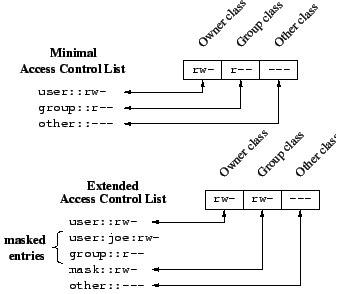
\includegraphics[width=0.5\textwidth]{Media/ACL.jpg}
    \caption{\Gls{ACL}}
    \label{fig:ACL}
\end{figure}
\subsubsection{\Gls{RBAC}}
Este esquema de seguridad está diseñado para organizaciones o sistemas en los que van a interactuar distintos usuarios con una gran cantidad de datos. El sistema defiende que, en lugar de tener una tabla por cada objeto, definiendo la forma que tienen los usuarios de interactuar con él, se deberían establecer una serie de transacciones, que dependiendo del rol serán distintas. Estas transacciones, una vez definidas cambian poco porque un usuario específico va a usar unos documentos específicos, dependiendo de la responsabilidad que tenga en la organización. En la imagen \ref{fig:RBAC} se puede ver claramente como dependiendo del rol vas a poder acceder a ciertos objetos.
\begin{figure}[H]
    \centering
    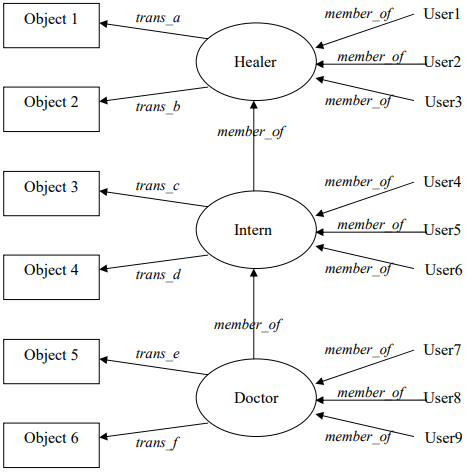
\includegraphics[width=0.5\textwidth]{Media/RBAC.PNG}
    \caption{\Gls{RBAC}}
    \label{fig:RBAC}
\end{figure}
Dos de las ventajas de este sistema son que cumplir el principio de de menor privilegio es relativamente sencillo, ya que se puede conseguir no proporcionándole  al usuario más transacciones de las que debe tener. Otra de las ventajas, innata, de \Gls{RBAC} es la separación de deberes. Esto es: En el caso de tener que realizar un transferencia bancaria, nunca se debería de poder proporcionar al mismo individuo el control de todo el flujo, ya que se le está dando la oportunidad de cometer algún tipo de irregularidad. Con RBAC puedes asignar dos transacciones, una que permita a un usuario solicitar una transferencia y otra que permita a un usuario validar la transferencia.
\subsubsection{\Gls{LDAP}}
Este protocolo está diseñado para permitir acceso a directorios complacientes con el estándar \Gls{X500} \textit{Directory Access Protocol} a sus usuarios. Uno de varios protocolos que tiene una aplicación para autenticarse con el fin de acceder al directorio \Gls{X500}\cite{LDAP}. La forma de acceder a los datos cambia según el protocolo de acceso a \Gls{X500}. Por ejemplo, en esta implementación, la forma de acceder a los datos sería:
\begin{verbatim}
	cn=Rosanna Lee, ou=People, o=Sun, c=us
\end{verbatim}
mientras que la implementación de Microsoft sería:
\begin{verbatim}
	/c=us/o=Sun/ou=People/cn=Rosanna Lee
\end{verbatim}
Cada uno de estos protocolos define una forma de "buscar" en \Gls{X500} información. Podemos ver que la implementación de \Gls{LDAP} está ordenada de derecha a izquierda, separada por el carácter (",") mientras que la implementación de Microsoft, \Gls{MAD} está ordenada de izquierda a derecha y separada con el carácter ("/").
Aunque no sea un método de autenticación que sucede en el mismo sistema, me parece que es lo suficientemente interesante como para incluirlo ya que es un ejemplo de autenticación en red.
\subsubsection{\Gls{SASL}}
Es un protocolo que proporciona métodos de añadir autenticación a protocolos de red mediante identificación y autenticación de los usuarios conectados al servidor. Además, gestiona el nivel de seguridad que se desea establecer para las futuras interacciones entre el servidor y el usuario conectado. Si se llega a la conclusión de que si que se requiere una capa de seguridad, esta se añade entre el propio protocolo y la conexión.\cite{rfc2222} 
Las distintas formas de autenticarse a un servidor con este protocolo son:
\begin{itemize}
	\item{\textbf{Anonymous: }}Usado para autenticar a clientes a servicios anónimos. El cliente envía un token (Correo electrónico) para permanecer identificado con el servidor. Es una forma sencilla y rápida de implementar, pero no es segura.
	\item{\textbf{CRAM-MD5: }}Usa el nombre de usuario y una contraseña para autenticar a los usuarios, pero solamente se transfiere la contraseña hasheada. Esto implica que no se pueden usar métodos de autenticación normal como \Gls{PAM}, que no soporta extracción de contraseñas. Es una forma simple y segura de autenticarse con el servidor.
	\item{\textbf{KERBEROS\_V4: }}Forma de autenticación fiable. Rápida, pero complicada de implementar. Muy segura.
	\item{\textbf{por defecto (autenticación y autorización): }}Usa el nombre de usuario y la contraseña para autenticar a los usuarios. La forma más rápida y sencilla pero poco segura.
	\item{\textbf{SCRAM-MD5: }}Deprecada.
	\item{\textbf{DIGEST-MD5: }}Basada en CRAM-MD5 pero da soporte a más características. Solo se transfieren las contraseñas hasheadas, por tanto no se puede usar \Gls{PAM} como backend. Es simple y seguro.
	\item{\textbf{LOGIN: }}Usa nombre de usuario y contraseña para autenticar a los usuarios. Rápida, simple de implementar pero nada segura.
	\item{\textbf{OTP: }}One Time Password
	\item{\textbf{SECURID: }}Usa una clave de un dispositivo hardware para autenticar a los usuarios. Buena velocidad, difícil de implementar pero buena seguridad.
\end{itemize}
Este protocolo ofrece una ventaja muy significativa. Proporciona a los desarrolladores la posibilidad de implementar su propio mecanismo para que utilice SASL.
\subsubsection{Kerberos}
Kerberos es un protocolo de autenticación de red diseñado para proporcionar un alto nivel de seguridad en la forma en la que el cliente y el servidor se autentican. Para conseguir esto, usa criptografía de llave secreta.\cite{mit-kerberos}\\El protocolo parte con la base de que internet no es un sitio seguro. Muchos protocolos ni siquiera usan algún tipo de seguridad. Existen herramientas con intención maliciosa para sacar las contraseñas de la red, por tanto, transferir credenciales descifradas a través de la red, es una práctica muy insegura. Algunas páginas usan \Gls{firewalls} para solucionar sus problemas de seguridad, pero los \Gls{firewalls} suponen que el problema está en el exterior cuando deberían asumir que se pueden vulnerar desde dentro también. Los firewalls, además los inconvenientes de los firewalls son inaceptables porque restringen la forma que tienen los usuarios de acceder a internet.\\Kerberos es la solución para este tipo de problemas de seguridad. El protocolo de kerberos usa una criptografía muy fuerte para que tanto el servidor como el cliente puedan comunicarse a través de una red insegura. Tras haberse autenticado mediante \Gls{kerberos} pueden cifrar la comunicación entre ellos.
\subsubsection{\Gls{NIS/NIS+}}
Proporciona información a los sistemas que tiene que tener para que cualquier usuario pueda autenticarse en cualquier sistema de esa misma red. Por tanto, debe mantener sincronizados y actualizados datos como:
\begin{itemize}
	\item Nombres de usuario, contraseñas y directorios principales de cada usuario (/etc/passwd)
	\item Información de grupos (/etc/group)
	\item Nombres de sistemas y direcciones IP (/etc/hosts)
\end{itemize}
Esta información la administra el servidor central. Dependiendo del tamaño de la red, el administrador de sistemas puede decidir replicarla en más ordenadores (esclavos) que se mantienen actualizados siempre con el servidor maestro (Cada vez que este se actualiza) Una de las ventajas de esto es que al estar los datos distribuidos, si se cae el servidor maestro, los usuarios de la red no sufren ningún percance, ya que la información está reflejada en los esclavos. Otra de las ventajas de mantener la información distribuida es que los esclavos también pueden responder a peticiones de clientes, por tanto, si un esclavo tarda menos en responder que el servidor, este puede facilitar la información al cliente.\\La diferencia entre NIS y NIS+ es que el último implementa muchas mejoras, incluida entre ellas, la posibilidad de tener dominios jerárquicos.\\Sin embargo, la mayor parte de administradores de sistemas recomendarían usar NIS, ya que es bastante más sencillo de administrar.
\subsubsection{\Gls{SSH}}
Una de las formas que han tenido los usuarios de conectarse de forma remota con un sistema ha sido el \Gls{telnet}. Esta opción, aunque válida, es poco segura porque la comunicación entre la máquina y el usuario se envía sin cifrar a través de la red.\\Se desarrolló SSH para evitar esto.

\subsubsection{\Gls{PAM}}
\section{conclusiones}
\clearpage
\printbibliography[heading=bibintoc,title={Bibliografía}]
\end{document}

